\subsection{Convex Optimization}

Convex optimization techniques can be applied to the spectral data to identify and quantify the contributions of different soil components. By formulating the problem as a convex optimization task, it is possible to find the optimal coefficients for the spectral components that minimize the difference between the observed and modeled spectra.

\begin{figure}[H]
\centering
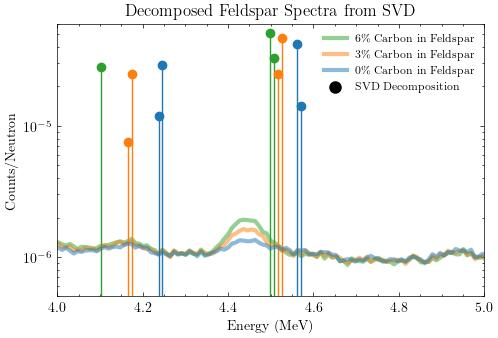
\includegraphics[width=0.8\textwidth]{../Figures/Analysis/decomposed_feldspar_svd.jpg}
\caption{Convex optimization process showing SVD decomposition of feldspar spectral data}
\label{fig:svd_decomposition}
\end{figure}

\begin{figure}[H]
\centering
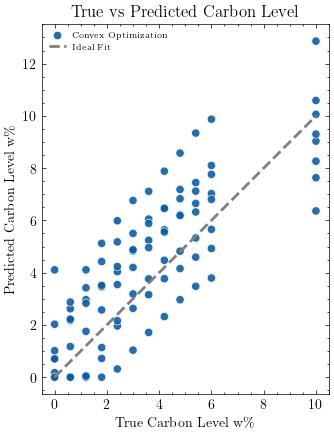
\includegraphics[width=0.8\textwidth]{../Figures/Analysis/carbon_level_vs_predicted_convex_optimization.jpg}
\caption{Convex optimization predictions showing carbon level vs predicted values using SVD}
\label{fig:svd_predictions}
\end{figure}